%!TEX root = ../main.tex
\subsection{Evalution of \texttt{GoodCore}$^+$}
\label{exp:sec:G+}

In this part, we compare \texttt{GoodCore}$^+$ solutions with \ours. For the hyperparameters, it's same as the Section~\ref{exp:sec:overall}.

\begin{figure*}
	\centering
	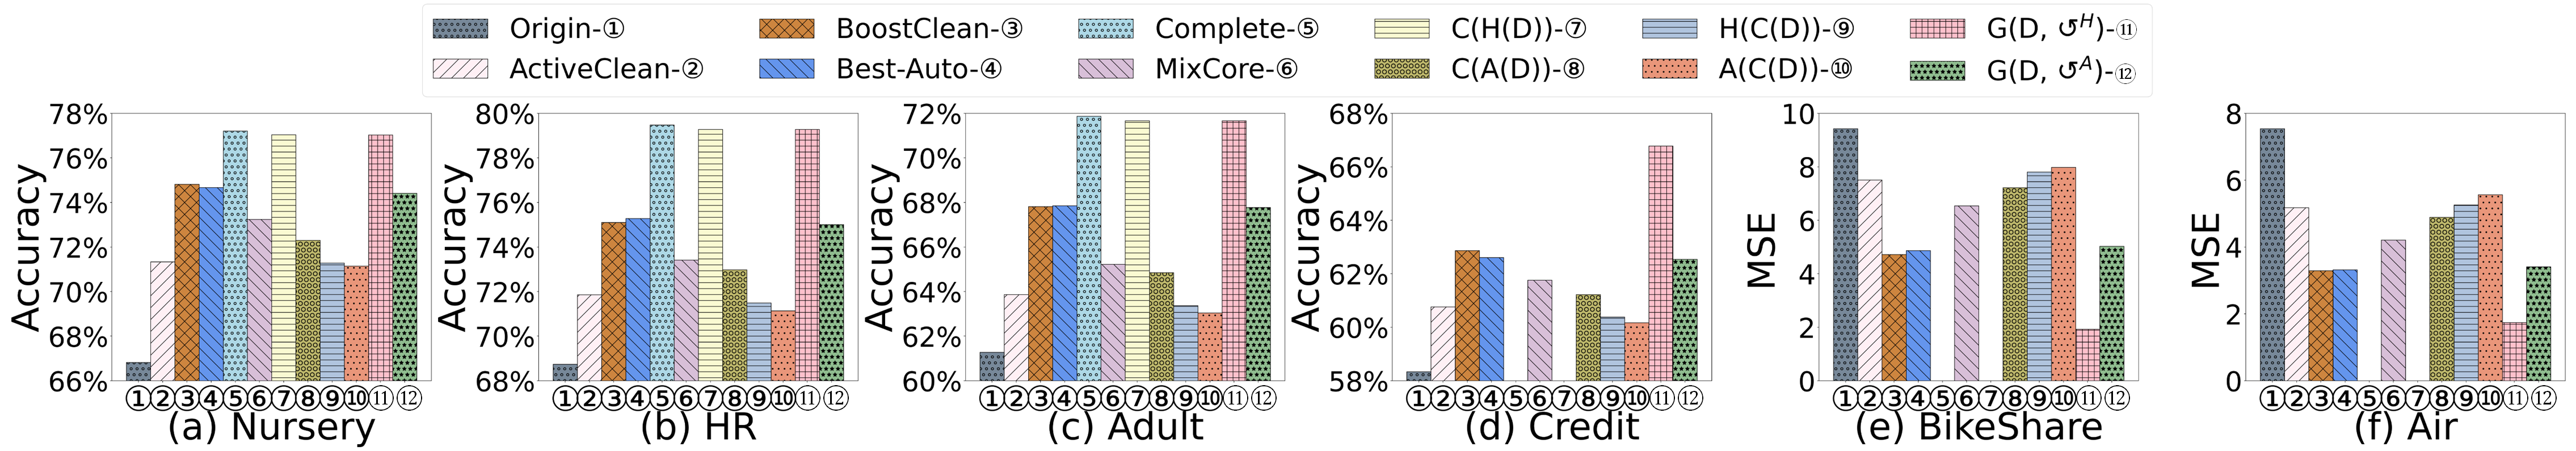
\includegraphics[width=\textwidth]{figs/effectiveness_new}
%	\vspace{-2.5em}
	\caption{Effectiveness of $G$ vs $G^+$.}
	\label{fig:effectiveness_new}
%	\vspace*{-1.2em}
\end{figure*}

\begin{figure*}
	\centering
	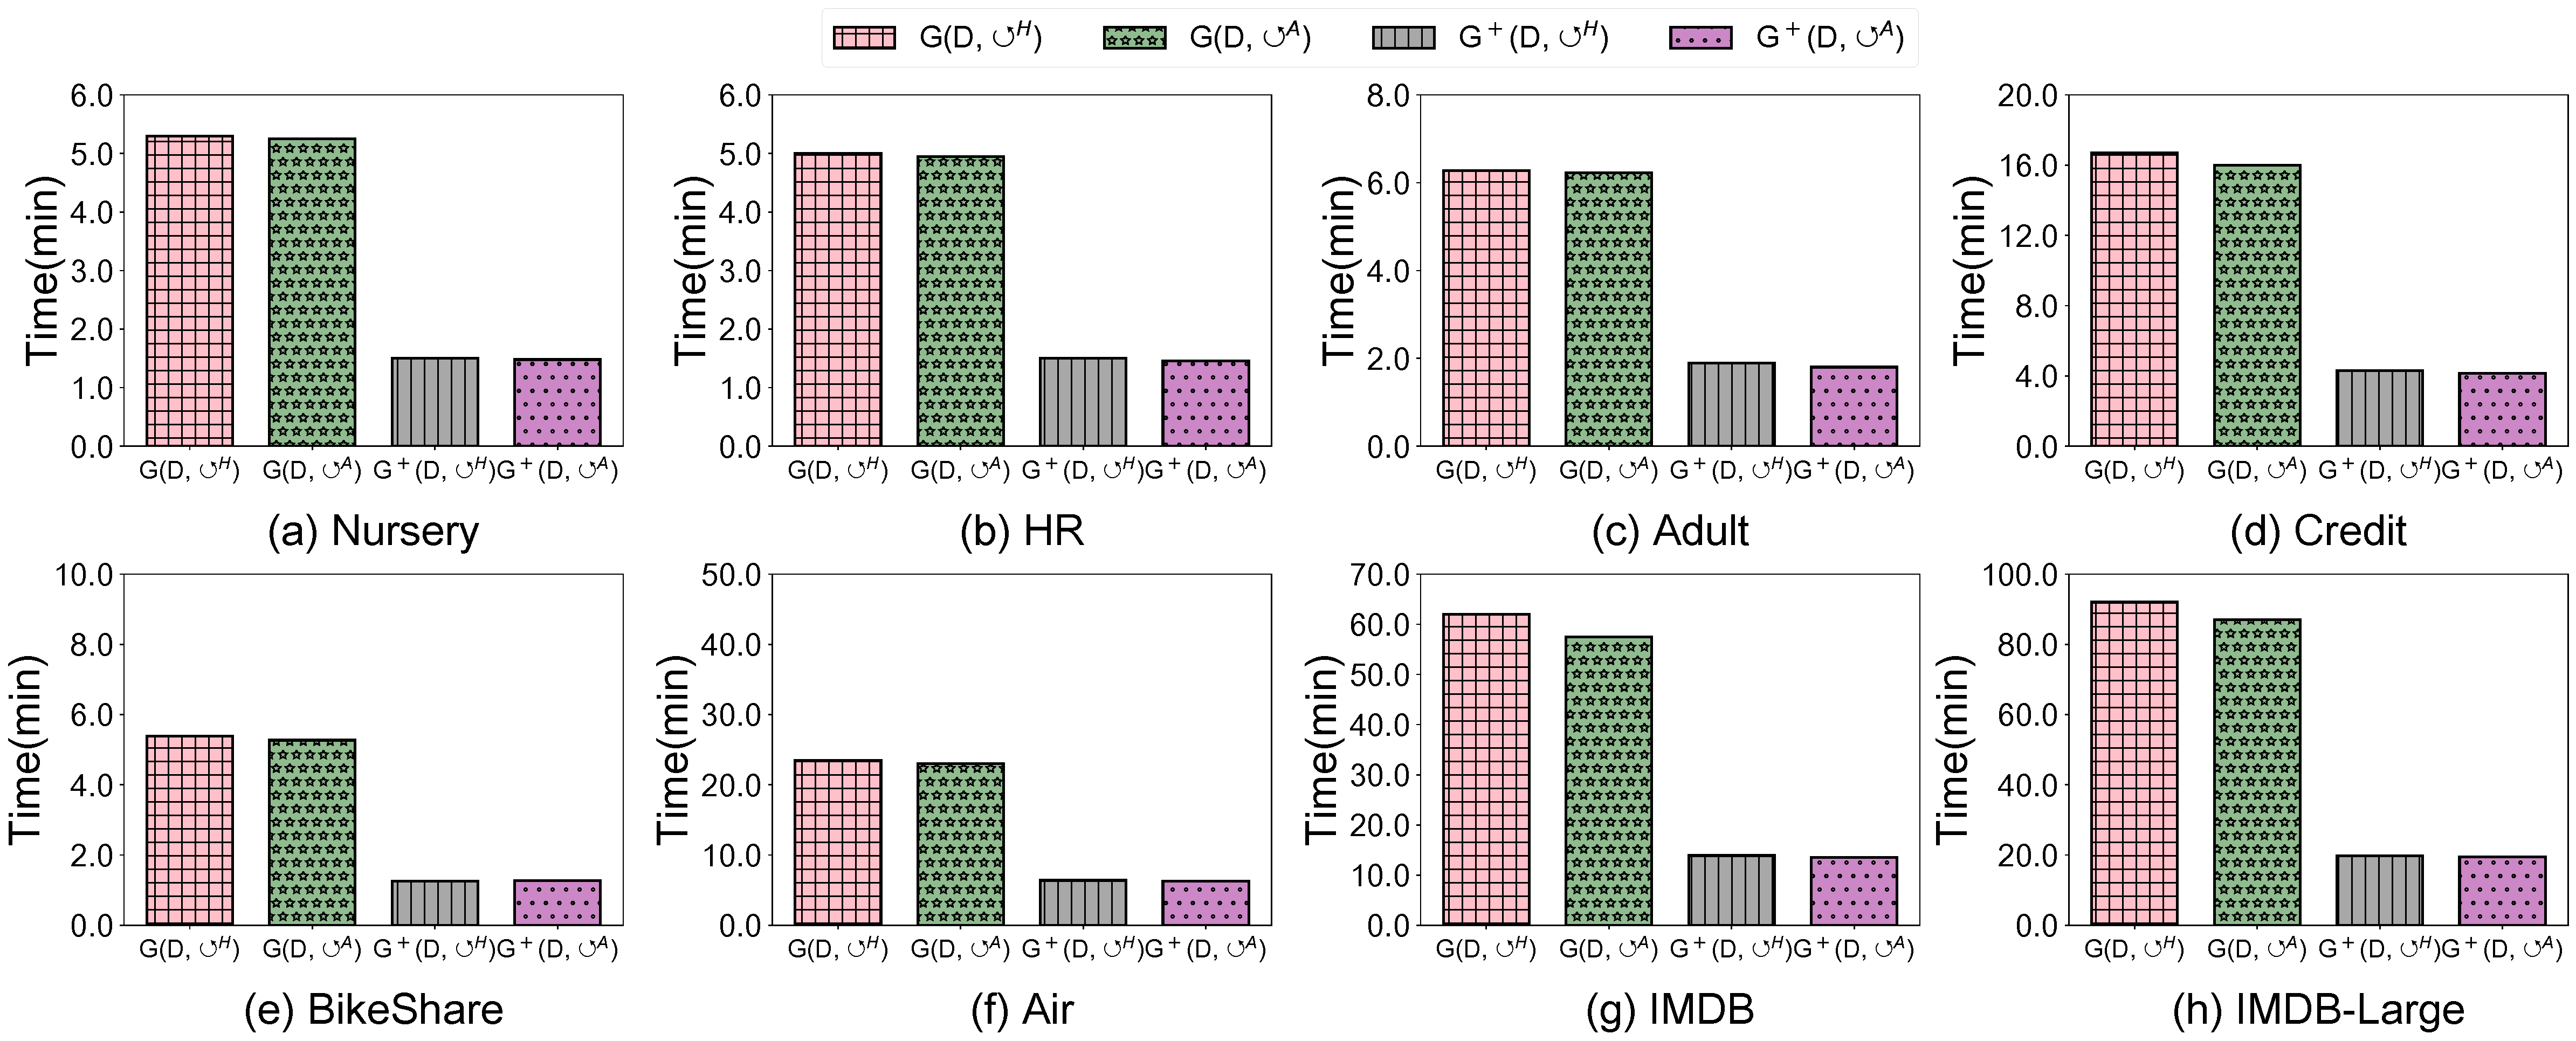
\includegraphics[width=\textwidth]{figs/efficiency_new}
%	\vspace{-2.5em}
	\caption{Efficiency of $G$ vs $G^+$. Note that only machine cost (i.e., runtime of machine) is considered.}
	\label{fig:efficiency_new}
%	\vspace*{-1.5em}
\end{figure*}


\subsubsection{Evaluation of model accuracy.}
The results are provided in Figure~\ref{fig:effectiveness_new}. We can found that the accuracy of \texttt{GoodCore}$^+$ and \ours are roughly the same on all datasets. For example, on dataset \imdbl,  $\nine$and $\seven$ achieve accuracy of 74.7\% and 74.9\% and they differ from each other by 0.2\%. This is because both of them   select a good coreset. In addition, we can observe that $\nine$ performs better than $\ten$ because human imputation is more accurate than automatic methods. For example, on \imdbl,  $\nine$ has an accuracy of 74.7\%, while $\eight$ is below 70\%.

\subsubsection{Evaluation of the efficiency.}~\label{sec:exp:efficiency_g} We  evaluate the efficiency of \texttt{GoodCore}$^+$ and \ours, including the machine cost and human cost.

\noindent{\bf Machine cost.} Machine cost is shown  in Figure~\ref{fig:efficiency_new}.  \texttt{GoodCore}$^+$ is more efficient than \ours. For example, on \imdbl, $\nine$ spends about 12min, which is $4.8\times$ (similar to $5\times$) faster than $\seven$. That is because $\nine$ have the lower time complexity than $\seven$, which is discussed in Section~\ref{subsec:pq}


\noindent{\bf Human cost.} In terms of the human cost, as shown in~Table~\ref{tbl:humancost}, $\nine$ and $\seven$ are cost-effective because humans just need to impute missing tuples in the much smaller coreset. For example, they only cost 520 and 511 tuples on dataset \imdbl respectively. 

\noindent \textbf{Summary.} 
Based on the results, we have the following conclusions. (1) Although we group tuples over the entire train set, our proposed methods $\nine$ and $\ten$ still achieve high  accuracy because the gradient approximation error can still be bounded. (2) The efficiency is much improved compared with \ours because we just need to iterate these groups rather than  the entire train set within the 3-loop coreset selection process. (3) The human cost is competitive with $\seven$ because the group-based solution has low impact on the number of tuples to be imputed by humans.

%(1) Our proposed methods $\nine$ and $\ten$ achieve high model accuracy due to the carefully selected coreset, which effectively represents the underlying ground truth through gradient approximation while considering potential repairs. Additionally, their practicality is evident through their low machine cost. (2) In comparison to $\seven$, the human cost associated with $\nine$ is significantly reduced, as demonstrated in Fig~\ref{fig:efficiency_new}, such as $11.9$min versus $57$min on the \imdbl dataset. Therefore, opting for $\nine$ is advisable when aiming for high model accuracy while managing a specific level of human cost. (3) Conversely, if neither accuracy nor human cost is a primary concern, the notably more efficient $\ten$ presents itself as an appealing option.